
\begin{frame}{Overview: Double Descent}
    The generalization error can be separated into bias and variance:
    \begin{align*}
        \mathcal{E}_{g} &= \mathbb{E}_{\vec{x},\mathcal{D}}\left[\left(f_\star(\vec{x}) - f_{\vec{\theta}}(\vec{x})\right)^2\right] \\
        &= \mathbb{E}_{\vec{x}}\left[\left(\eqhl{teal}{\mathrm{Bias}(f_{\vec{\theta}},\vec{x})}\right)^2 + \eqhl{red}{\mathrm{Var}\left(f_{\vec{\theta}}(\vec{x})\right)}\right] \\
        &= \mathbb{E}_{\vec{x}}\left[\left(\eqhl{teal}{f_{\star}(\vec{x}) - \mathbb{E}_{\mathcal{D}}\left[f_{\vec{\theta}}(\vec{x})\right]}\right)^2 + \eqhl{red}{\mathbb{E}_{\mathcal{D}}\left[\left(f_{\vec{\theta}}(\vec{x}) - \mathbb{E}_{\mathcal{D}}\left[f_{\vec{\theta}}(\vec{x})\right]\right)^2\right]}\right]
    \end{align*}

    \vspace{-0.7cm}
    
    \begin{figure}
        \centering
        % \begin{tikzpicture}
        %     \draw[->] (0, 0) -- (6, 0) node[right] {$x$};
        %     \draw[->] (0, 0) -- (0, 3) node[above] {$y$};
        %     \draw[scale=0.5, domain=-3:3, smooth, variable=\x, blue] plot ({\x}, {\x*\x});
        %     \draw[scale=0.5, domain=-3:3, smooth, variable=\y, red]  plot ({\y*\y}, {\y});
        % \end{tikzpicture}
        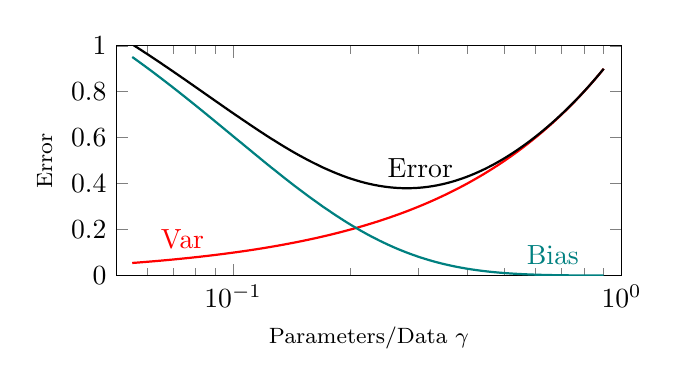
\begin{tikzpicture}
        \begin{axis}[
            width = 8cm, height = 4.5cm,
            xmax = 1, xmin = 0.05, xmode = log, xlabel = {\footnotesize Parameters/Data $\gamma$},
            ymax = 1, ymin = 0, ymode = normal, ylabel = {\footnotesize Error}
        ]
        \addplot[
            domain=0.055:0.9, 
            samples=100, 
            color=red,
            thick,
        ]
        {x}
        node[pos=0.1,above] {Var};
        \addplot[
            domain=0.055:0.9, 
            samples=100, 
            color=teal,
            thick,
        ]
        {exp(-10 * (x - 0.05))}
        node[pos=0.9,above] {Bias};
        \addplot[
            domain=0.055:0.9, 
            samples=100, 
            color=black,
            thick,
        ]
        {exp(-10 * (x - 0.05)) + x}
        node[pos=0.6,above] {Error};
        \end{axis}
        \end{tikzpicture}
    \end{figure}
\end{frame}

\begin{frame}{Overview: Double Descent}
    Model performances are not trivial:
    \begin{figure}
        \centering
        \includegraphics[width = 0.8\textwidth]{figures/double_descent.png}
        \begin{tikzpicture}[overlay,remember picture,>=stealth,nodes={align=left,inner ysep=1pt},<-]
            \draw[draw=white,fill=white] (-3.2,0.4) rectangle (-2.9,0.0) node[pos=0.4] {\tiny$\gamma$};
        \end{tikzpicture}
        \credit{Rocks et al. '22}
    \end{figure}
    This is the \hl{double descent} behavior.
    \begin{itemize}
        \item Behavior depends on the \hl{hyperparameters}.
        \item Explain via neural tangent kernel (NTK), $\Theta_0$.
    \end{itemize}
\end{frame}

\begin{frame}{Overview: Replica Trick}
    Using the \hl{replica trick}, we will be able to derive the following double descent curve for ridgeless kernel regression.

    \begin{figure}
        \centering
        \includegraphics[width=0.9\linewidth]{figures/doubleDescent1.pdf}
    \end{figure}
\end{frame}


% \begin{frame}{Overview: Spectral Mode}
%     Along the way, we see
% \end{frame}

% \begin{frame}{Overview: Feature Learning}    
% \end{frame}